\documentclass[11pt]{article}
% Basic Packages for Encoding (Input AND Output) and Langauge Support
\usepackage[utf8]{inputenc}
\usepackage[T1]{fontenc}
\usepackage[french]{babel}

% Change Layout with a User-Friendly Interface
\usepackage[margin=1in]{geometry}

% Include Pictures with a User-Friendly Interface
\usepackage{graphicx}
\usepackage{float}

% Extended Math Support from the Famous 'American Mathematical Society'
\usepackage{amsmath}
\usepackage{amsfonts}
\usepackage{amssymb}

% For the chemistry
\usepackage{chemist}

% Just for Demonstration Purposes
\usepackage[math]{blindtext}

% For use on computer
\usepackage{hyperref}

% For table color
\usepackage{xcolor,colortbl}

% Titre
\usepackage[affil-it]{authblk}
\title{\textbf{TP Détermination d'une masse molaire atomique}}
\author{Manon Bruno, Romain Blondel}
\affil{2M8, Gymnase Auguste Piccard}

\begin{document}
\maketitle

\section{But}
Produire et mesurer un volume de dihydrogène, déterminer la quantité de dihydrogène produite en mole et calculer la masse molaire atomique du magnésium utilisé dans la réaction.

\section{Introduction}
Cette expérience présente une façon assez simple de mesurer la masse molaire d'un élément. Cela est utile pour établir des tables et dans le cadre de divers calculs afin de les réutiliser dans d'autres situations plus complexes ou à des fins prédictive, par exemple dans l'industrie.\\
Pour cette expérience, nous avons fait réagir du magnésium avec une solution d'acide chlorhydrique 2M ce qui produit du chlorure de magnésium et du dihydrogène. La formule de la réaction est:
\begin{chemeqn}
2HCl_{(l)} + Mg_{(s)} \longrightarrow MgCl_{2(aq)} + H_{2(g)}
\label{eq:react}
\end{chemeqn}
Afin de mesurer le volume de \chemform{H_2}, on fait une simplification à l'aide de la loi des gaz parfaits, plus précisément la formule:
\begin{equation}
P \cdot V = n \cdot R \cdot T
\label{eq:gaz-parfaits}
\end{equation}
où P est la pression en kilopascals, V le volume en litre, n la quantité de gaz en mole, R la constante des gaz parfaits qui vaut $\sim 8,31 \left[ \frac{kPa \cdot L}{mol \cdot K} \right]$ et T la température absolue en Kelvin.
Cette loi est un modèle qui, en se basant sur le comportement observé des gaz à basse pression, simplifie ces comportements en les décrivant comme identiques. Ce modèle a été confirmé par la théorie cinétique des gaz qui admet plusieurs hypothèses dont certaines seront évoquées au court de la discussion.

\section{Principe de mesure et description}
\subsection{Montage}
\begin{figure}[H]
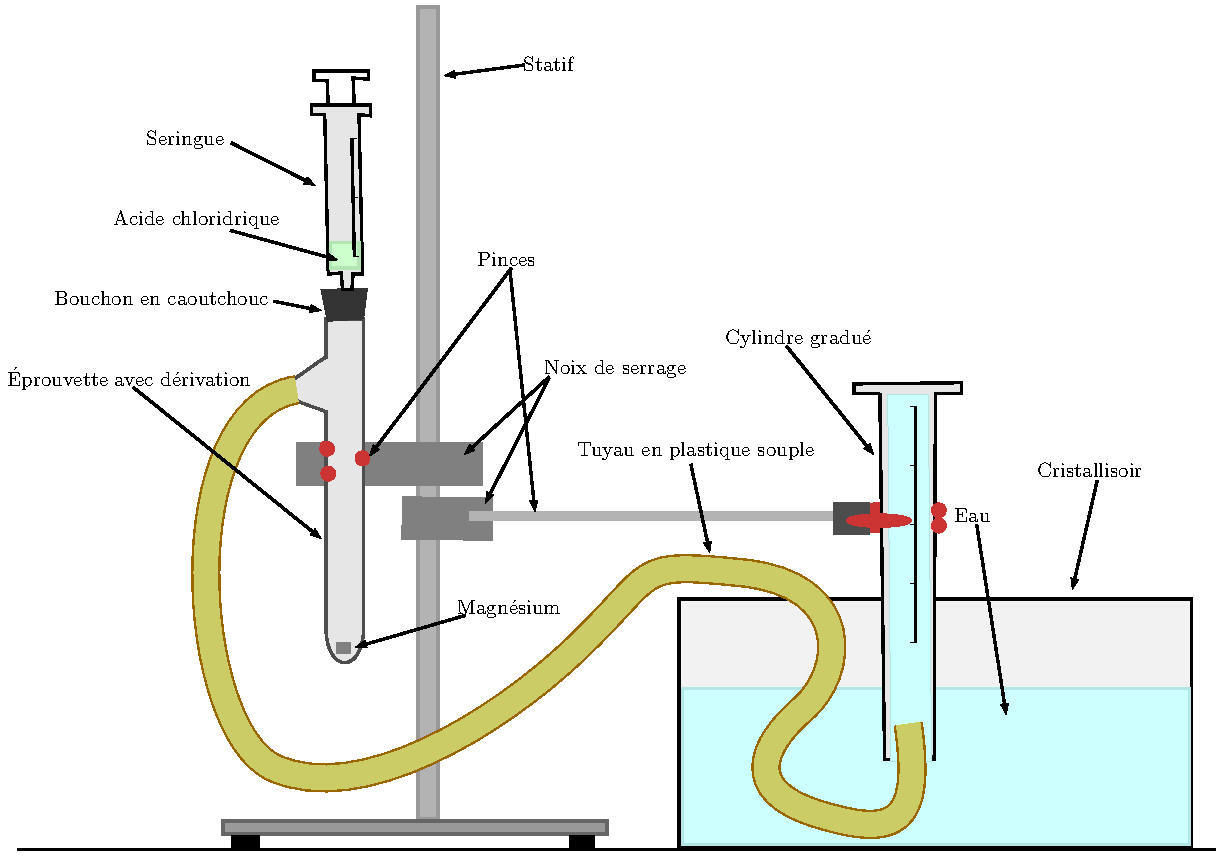
\includegraphics[scale=0.8]{schema-montage.pdf}
\caption{Schéma du montage}
\label{figure:schem-montage}
\end{figure}

\subsection{Mode opératoire}
\begin{enumerate}
\item Prendre une éprouvette avec dérivation de 150 [mL] et la placer dans une pince, elle-même fixée sur un statif
\item Ajouter un tuyeau en plastique souple sur la dérivation
\item Prendre un cristallisoir ainsi qu'un cylindre gradué de 25 [mL] et s'assurer que le cylindre peut se placer en position couchée dans le cristallisoir
\item Remplir le cristallisoir au 2/3 d'eau
\item Placer le cylindre gradué à l'envers avec l'ouverture immergée dans l'eau et l'immobiliser à l'aide d'une autre pince fixée au statif après s'être assuré qu'il ne contenait pas de bulles d'air
\item Couper un segment de rouleau de magnésium de maximum 0,5 [cm] et le peser avant de le placer dans l'éprouvette avec dérivation
\item Placer un bouchon en caoutchouc au bout d'une seringue et la remplir d'environ 10 [mL] d'acide chlorhydrique 2M. Penser à mesurer la quantité d'acide dans la seringue et celle d'air
\item Fermer l'éprouvette avec dérivation avec la seringue et le bouchon puis vider l'acide chlorhydrique
\item Mesurer la quantité de dihydrogène se retrouvant piégée dans le cylindre gradué
\end{enumerate}

\section{Résultats}
Tout d'abord, les mesures données par des sources externes sont la température du laboratoire de $T_{lab} = 20.5 [^\circ C] = 293.65 [K]$ et la pression du jour (donnée sur un \href{https://meteolausanne.com/pression}{site de météo}) $P_{atm} = 1014.15 [hPa] = 101.415 [kPa]$. Nous avons mesuré ensuite le volume dans le seringue (air et acide ainsi que acide seul) ainsi que le volume d'air dans l'éprouvette et la masse de magnésium (voir table \ref{table:mesures}). Le morceau de magnésium pour la première mesure est long de $0.5 [cm]$ et de $0.4 [cm]$ pour la seconde.

\begin{table}[H]
\center
\begin{tabular}{|>{\columncolor{gray}}c||c|>{\columncolor{lightgray}}c|c|>{\columncolor{lightgray}}c|}
\hline
\rowcolor{gray} \cellcolor{black} & $V_{seringue} [mL]$ & $V_{acide} [mL]$ & $V_{\acute{e}prouvette} [mL]$ & $M_{Mg} [g]$ \\ \hline
Mesure 1 & $8.0$ & $6.0$ & $13.5$ & $0.009$ \\ \hline
Mesure 2 & $8.0$ & $6.0$ & $14.0$ & $0.008$ \\ \hline
\end{tabular}
\caption{Mesures}
\label{table:mesures}
\end{table}

\section{Calculs}
\subsection{Masse molaire atomique}
Pour calculer la masse molaire atomique du magnésium, il faut connaître le nombre de mole car sa masse est déjà mesurée. En voyant que la solution finale dans l'éprouvette à dérivation est homogène et de part la grande quantité d'acide injectée, on peut considérer la réaction comme complète et donc que le magnésium est complètement dissout. De fait et part l'équation chimique (\ref{eq:react}), on peut conclure que le nombre de mole du magnésium est égal à celui de dihydrogène. Pour calculer ce dernier, on peut connaître le volume de dihydrogène en soustrayant le volume totale dans l'éprouvette renversée par celui ajouté via la seringue : $V_{H_2} = V_{\acute{e}prouvette} - V_{seringue}$. De là, par la loi des gaz parfait (\ref{eq:gaz-parfaits}) on obtient le nombre de mole de dihydrogène par $P \cdot V = n \cdot R \cdot T \Leftrightarrow n = \frac{P \cdot V}{R \cdot T}$ (car T et P sont mesurés et R est une constante). Finalement, il ne reste plus qu'à calculer la masse molaire atomique du magnésium $MM_{Mg} = \frac{M_{Mg}}{n_{Mg}}$. Les valeurs numériques sont donc résumée dans la table \ref{table:res-exp-ini}.

\begin{table}[H]
\center
\begin{tabular}{|>{\columncolor{gray}}c||c|>{\columncolor{lightgray}}c|c|}
\hline
\rowcolor{gray} \cellcolor{black} & $V_{H_2} [mL]$ & $n_{H_2} = n_{Mg} [mol]$ & $MM_{Mg} [\frac{g}{mol}]$ \\ \hline
Mesure 1 & $5.5$ & $2.28 \cdot 10^{-4}$ & $39.393$ \\ \hline
Mesure 2 & $6.0$ & $2.49 \cdot 10^{-4}$ & $32.098$ \\ \hline
\end{tabular}
\caption{Calculs de $MM_{Mg}$}
\label{table:res-exp-ini}
\end{table}

\subsubsection*{En ne considérant que l'acide}
Au vu des résultats, il est à craindre une erreur non  négligeable. Il est donc curieux de voir qu'est-ce que cela donne si l'on prend comme volume injecté uniquement celui d'acide, et non pas avec l'air également présent dans la seringue. Cela donne la table \ref{table:res-exp-2}.

\begin{table}[H]
\center
\begin{tabular}{|>{\columncolor{gray}}c||c|>{\columncolor{lightgray}}c|c|}
\hline
\rowcolor{gray} \cellcolor{black} & $V_{H_2} [mL]$ & $n_{H_2} = n_{Mg} [mol]$ & $MM_{Mg} \left[\frac{g}{mol}\right]$ \\ \hline
Mesure 1 & $7.5$ & $3.115 \cdot 10^{-4}$ & $28.888$ \\ \hline
Mesure 2 & $8.0$ & $3.323 \cdot 10^{-4}$ & $24.073$ \\ \hline
\end{tabular}
\caption{Calculs de $MM_{Mg}$ en ne considérant pas le volume d'air dans la seringue}
\label{table:res-exp-2}
\end{table}

\subsection{Erreur}
Avec la valeur théorique de la masse molaire atomique dans le tableau périodique $u_{Mg} = 24.305 \left[\frac{g}{mol}\right]$, il est intéressant d'établir des tables d'erreur. Celle absolue se calcule en faisant la différence entre la valeur théorique et celle mesurée $\Delta x = | v_{th} - v_{mes}|$. Quand à l'erreur relative c'est le quotient entre celle absolue et la valeur théorique $\frac{\Delta x}{x} = \frac{| v_{th} - v_{mes}|}{v_{th}}$. Le tout est résumé dans les table \ref{table:err-exp-ini} et \ref{table:err-exp-2}.

\begin{table}[H]
\center
\begin{tabular}{|>{\columncolor{gray}}c||c|>{\columncolor{lightgray}}c|}
\hline
\rowcolor{gray} \cellcolor{black} & $\Delta x \left[\frac{g}{mol}\right]$ & $\frac{\Delta x}{x} [\%]$ \\ \hline
Mesure 1 & $15.09$ & $62.08$ \\ \hline
Mesure 2 & $7.79$ & $24.28$ \\ \hline
\end{tabular}
\caption{Erreur sur $MM_{Mg}$}
\label{table:err-exp-ini}
\end{table}

\subsubsection*{En ne considérant que l'acide}

\begin{table}[H]
\center
\begin{tabular}{|>{\columncolor{gray}}c||c|>{\columncolor{lightgray}}c|}
\hline
\rowcolor{gray} \cellcolor{black} & $\Delta x \left[\frac{g}{mol}\right]$ & $\frac{\Delta x}{x} [\%]$ \\ \hline
Mesure 1 & $4.58$ & $18.86$ \\ \hline
Mesure 2 & $0.23$ & $0.96$ \\ \hline
\end{tabular}
\caption{Erreur sur $MM_{Mg}$ avec la variante de calcul}
\label{table:err-exp-2}
\end{table}

\section{Discussion}
Nous constatons, en suivant le protocole et les hypothèse d'origine, une erreur non négligeable, mais celle-ci est également présente entre les différentes itérations de l'expérience. De fait, nous allons principalement discuter de ces points car la valeur dans les tables doit être considérée comme fiable. \\ \\
Tout d'abord, la différence entre les deux mesures peut s'expliquer de différentes manières. La plus évidente est celle liée à l'observateur. En effet, les mesures de volumes sont effectuées à l’œil et sont donc soumises à une incertitude. Ensuite, les appareils de mesure ne sont pas les plus adaptés. La balance est précise au centième de gramme ce qui nous donnent des mesures à 1 chiffre significatif, ainsi que des valeurs un peu oscillantes affichées dans nos deux mesures. La seringue n'étant pas calibrée à volume fixe, mais juste remplie puis utilisée, la mesure des différents volumes injectés est assez approximative. Finalement, le cylindre renversé n'est pas prévu pour cette utilisation dans son marquage et donc dans la manière qu'on a de le lire. Il faut aussi noter la présence de bulles d'air dans ce dernier qui impacte la mesure puis le calcul du volume de dihydrogène. \\ \\
Pour les erreurs vis-à-vis de la valeur théorique, outre les mêmes problèmes que sur la mesure, il y a des facteurs possibles sur le modèle utilisé ainsi que l'interprétation des résultats. Premièrement, on peut noter que le magnésium est probablement en petite partie oxydé, ce qui fait que le nombre d'atomes régissant avec l'acide est moindre, ce qui rend la masse utilisée pour calculer la masse molaire légèrement supérieur donnant des masses molaires plus petites et donc proches de la valeur théorique (dans le cas de la seconde mesure, la balance oscillait entre 0.008 et 0.009 [g] avant de se stabiliser à 0.008 [g] ce qui laisse penser que ce facteur a en partie été compensé et cela se voit dans l'erreur ; il est importants de noter ce phénomène sur la mesure 1 également, et après calcul, si l'on utilisait 0.008 [g] on obtiendrait une erreur de presque 20 [\%] de moins). \\
Ensuite, dans le dispositif expérimental, quand le gaz remplace l'eau, tant que son niveau est au-dessus de celui de l'eau, la pression qu'il exerce va être très proche de celle de l'air, quoique légèrement faussée par l'eau qui exerce une certaine pression et qui est un contenant relativement déformable par la quantité de gaz. De fait l'application de la théorie des gaz parfaits demeure une approximation. De plus, si le niveau de gaz dans le cylindre passe en dessous de celui de l'eau, la pression de l'eau va augmenter celle dans le cylindre. Dans les deux cas, on obtient une pression un peu plus grande que celle de l'air dans le cylindre, ce qui permet une réflexion similaire à l'impacte de la masse de magnésium sur la masse molaire. Il faut également préciser que les mesures de température et de pression sont faites par rapport à une région sensiblement plus grande que le système expérimental (le laboratoire pour la température, respectivement la suisse romande pour la pression). \\
Finalement, le volume injecté dans le système par la seringue est discutable. Si on considère que quand on presse, le mouvement du joint permet à l'air resté dans la seringue de partir car bloqué par l'acide qui doit s'écouler, on pourrait omettre le volume d'air dans le volume injecté et ne considérer que celui d'acide. En faisant les calculs selon cette hypothèse, l'erreur baisse drastiquement (voir tables \ref{table:err-exp-ini} et \ref{table:err-exp-2}). Soit cette hypothèse est correcte, soit elle permet dans le cas de nos mesures de compenser les sources d'erreurs mentionnées plus haut. \\ \\
Pour conclure, nous avons à faire à un système très sensible à la mesure. Il suffit de voir les deux itérations à paramètres initiaux proches et leur différence d'erreur. Au vu de nos résultats, afin d'obtenir la valeur la plus proche possible de celle théorique, il serait intéressant de faire un arrondi "bas" pour la masse de magnésium et "haut" pour le volume de dihydrogène.


\section{Conclusion}
En conclusion, on peut constater que la seconde expérience est plus précise que la première. Étant donné que les différentes variables sont presque semblables, on peut penser que la différence vient d'une manipulation. Des pistes d'amélioration seraient de normaliser la pression du système qui est légèrement différente dans le cylindre gradué ou d'avoir un cylindre gradué plus grand afin que l'air reste au dessus du niveau de l'eau. On peut aussi agrandir le cristallisoir pour pouvoir retirer plus facilement les bulles d'air dans le cylindre. On pourrait avoir des instruments de mesure plus précis tel que la seringue, le cylindre gradué ou la balance. Dans le cas des 2 premiers, la mesure du volume est difficile et avoir un contenant plus adapté à la lecture de volume à l'envers que le cylindre gradué aiderait. Pour la balance, il serait plus intéressant qu'elle mesure du centième de gramme au dix-millième. Si on arrivait à retirer l'oxyde du magnésium, les mesures deviendraient aussi plus précise. Il pourrait aussi être intéressant d'utiliser une autre théorie que celle des gaz parfaits car, bien qu'elle permette de négliger les bulles d'aires, elle est basée sur des hypothèses qui ne sont pas toutes respectées dans l'expérience. Mais cela reste malgré tout une expérience intéressante pour estimer la masse molaire d'un matériau.

\end{document}